% SC1007 — Chapter 6: Hashing
% No \documentclass — included by modules/SC1007/main.tex (book class).
\chapter{Hashing}
\label{ch:hashing}

\begin{quote}
\emph{``Hashing is the closest we get to $O(1)$ search.''} --- If the hash behaves, the dictionary flies.
\end{quote}

\noindent\textbf{Prerequisites:} Ch.~1 (arrays), Ch.~5 (analysis). Hashing gives expected $O(1)$ insert/search/delete with high probability.

\section*{Learning Outcomes}
After this chapter you will be able to:
\begin{enumerate}[label=(L\arabic*)]
    \item design hash functions and explain universal hashing;
    \item implement chaining and analyse $O(1+\alpha)$ expected cost;
    \item implement open addressing (linear/quadratic/double hashing) and analyse clustering;
    \item handle load factor, rehashing, and deletion correctly.
\end{enumerate}

% ============================================================
\section{Hash Functions}
\label{sec:hash-functions}
A hash function $h:U\to\{0,\ldots,m-1\}$ maps universe $U$ into $m$ slots. Ideal: uniform, deterministic, fast. Two classic constructions for integer keys:

\begin{align}
h(k) &= k \bmod m \quad\text{(division, $m$ prime away from powers of 2)}, \nonumber\\
h(k) &= \lfloor m\cdot(kA\bmod 1)\rfloor \quad\text{(multiplication, $0<A<1$)}, \nonumber\\[4pt]
h(k) &= ((ak+b)\bmod p)\bmod m \quad\text{(universal family, $p$ prime $> |U|$)}. \nonumber
\end{align}

Universal hashing picks $a,b$ randomly at runtime, guaranteeing low collision probability for any adversarial input set.

\textbf{Strings:} polynomial rolling hash $h(s)=\sum_{i} s_{i}\cdot B^{i}\bmod m$ or Python's salted hash.

\begin{figure}[h]
\centering
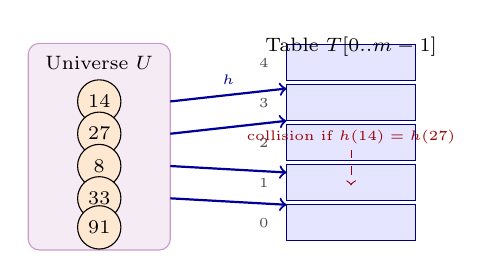
\begin{tikzpicture}[scale=0.82, every node/.style={font=\scriptsize}]
  % Universe -> slots
  \draw[fill=violet!8, draw=violet!40, rounded corners=4pt] (0,0) rectangle ++(2.2,3.2);
  \node at (1.1,2.9) {Universe $U$};
  \foreach \y/\k in {2.3/14,1.8/27,1.3/8,0.8/33,0.35/91} {
    \node[circle, fill=orange!18, draw, inner sep=1pt, minimum size=0.55cm] at (1.1,\y) {\k};
  }
  \draw[->, thick, blue!60!black] (2.2,2.3) -- (4.0,2.5) node[midway, above, font=\tiny] {$h$};
  \draw[->, thick, blue!60!black] (2.2,1.8) -- (4.0,2.0);
  \draw[->, thick, blue!60!black] (2.2,1.3) -- (4.0,1.2);
  \draw[->, thick, blue!60!black] (2.2,0.8) -- (4.0,0.7);
  % Table slots
  \foreach \i in {0,1,2,3,4} {
    \draw[fill=blue!10, draw=blue!50!black] (4.0,\i*0.62+0.15) rectangle ++(2.0,0.55);
    \node[font=\tiny, gray!60!black] at (3.65,\i*0.62+0.42) {\i};
  }
  \node at (5.0,3.15) {Table $T[0..m-1]$};
  % Collision annotation
  \node[font=\tiny, red!60!black] at (5.0,1.75) {collision if $h(14)=h(27)$};
  \draw[->, red!60!black, dashed] (5.0,1.55) -- (5.0,1.0);
\end{tikzpicture}
\caption{Hash function maps many keys into $m$ slots. Collisions are inevitable when $|U|>m$ (pigeonhole) and must be resolved.}
\label{fig:hash-map}
\end{figure}

% ============================================================
\section{Chaining}
\label{sec:chaining}
Each slot $T[j]$ holds a linked list (chain) of keys hashing to $j$. Load factor $\alpha=n/m$.

\begin{figure}[h]
\centering
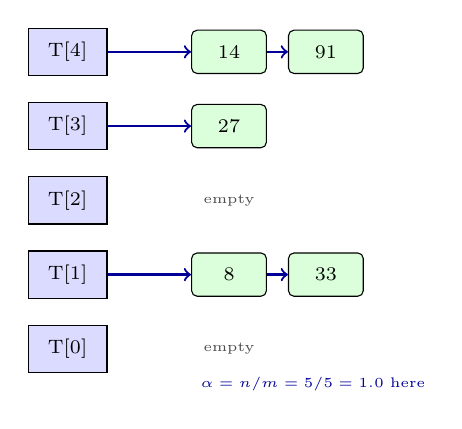
\begin{tikzpicture}[scale=0.82, every node/.style={font=\scriptsize},
  slot/.style={draw, fill=blue!14, minimum width=1.0cm, minimum height=0.60cm},
  cnode/.style={draw, fill=green!14, minimum width=0.95cm, minimum height=0.55cm, rounded corners=2pt}]
  \foreach \i in {0,1,2,3,4} {
    \node[slot] (s\i) at (0,\i*1.15) {T[\i]};
  }
  % Chains
  \node[cnode] (a) at (2.5,4*1.15) {14};
  \node[cnode] (b) at (4.0,4*1.15) {91};
  \draw[->, thick, blue!60!black] (s4.east) -- (a.west);
  \draw[->, thick, blue!60!black] (a.east) -- (b.west);
  \node[cnode] (c) at (2.5,3*1.15) {27};
  \draw[->, thick, blue!60!black] (s3.east) -- (c.west);
  \node[cnode] (d) at (2.5,1*1.15) {8};
  \node[cnode] (e) at (4.0,1*1.15) {33};
  \draw[->, thick, blue!60!black] (s1.east) -- (d.west);
  \draw[->, thick, blue!60!black] (d.east) -- (e.west);
  % Empty slots
  \node[font=\tiny, gray!60!black] at (2.5,2*1.15) {empty};
  \node[font=\tiny, gray!60!black] at (2.5,0) {empty};
  \node[font=\tiny, blue!60!black] at (3.8,-0.55) {$\alpha=n/m=5/5=1.0$ here};
\end{tikzpicture}
\caption{Chaining: each slot heads a linked list. Expected chain length $=\alpha$; search scans the chain.}
\label{fig:chaining}
\end{figure}

Under \emph{simple uniform hashing}, expected search cost is $\Theta(1+\alpha)$ (hash + chain scan). If $m=\Theta(n)$ then $\alpha=O(1)$ and operations are expected $O(1)$. Worst case $\Theta(n)$ if all keys collide, but universal hashing makes this vanishingly unlikely.

\begin{lstlisting}[language=Python]
# Chaining -- Python sketch
class ChainedHash:
    def __init__(self, m=8):
        self.m = m
        self.T = [[] for _ in range(m)]
    def _h(self, k): return hash(k) % self.m
    def insert(self, k, v):
        b = self._h(k)
        for i,(kk,_) in enumerate(self.T[b]):
            if kk == k: self.T[b][i]=(k,v); return
        self.T[b].append((k,v))
    def search(self, k):
        for kk,v in self.T[self._h(k)]:
            if kk == k: return v
        return None
\end{lstlisting}

Rehashing: when $\alpha$ exceeds threshold (e.g.\ $0.75$), allocate $2m$ slots and reinsert all keys: $O(n)$ but amortised $O(1)$.

% ============================================================
\section{Open Addressing}
\label{sec:open-addressing}
All keys live in $T$ itself. Probe sequence $h(k,0),h(k,1),\ldots,h(k,m-1)$ is a permutation of slots.

\begin{itemize}
    \item \textbf{Linear probing:} $h(k,i)=(h(k)+i)\bmod m$. Suffers \emph{primary clustering} (long runs).
    \item \textbf{Quadratic probing:} $h(k,i)=(h(k)+c_{1}i+c_{2}i^{2})\bmod m$. Reduces primary clustering.
    \item \textbf{Double hashing:} $h(k,i)=(h_{1}(k)+i\cdot h_{2}(k))\bmod m$. Best distribution; $h_{2}(k)\neq0$.
\end{itemize}

\begin{figure}[h]
\centering
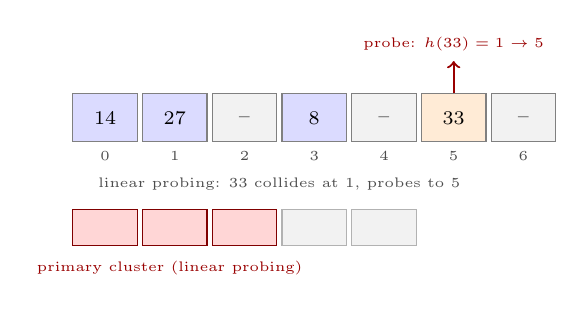
\begin{tikzpicture}[scale=0.82, every node/.style={font=\scriptsize}]
  \foreach \i/\v/\c in {0/14/blue!14,1/27/blue!14,2/--/gray!10,3/8/blue!14,4/--/gray!10,5/33/orange!16,6/--/gray!10} {
    \draw[fill=\c, draw=black!50] (\i*1.08,0) rectangle ++(1.0,0.75);
    \node at (\i*1.08+0.5,0.37) {\v};
    \node[font=\tiny, gray!60!black] at (\i*1.08+0.5,-0.22) {\i};
  }
  \draw[->, thick, red!60!black] (5*1.08+0.5,0.75) -- ++(0,0.5) node[above, font=\tiny] {probe: $h(33)=1\to5$};
  \node[font=\tiny, gray!60!black] at (3.2,-0.65) {linear probing: 33 collides at 1, probes to 5};
  % Clustering illustration
  \begin{scope}[yshift=-1.6cm]
    \foreach \i in {0,1,2} {
      \draw[fill=red!16, draw=red!50!black] (\i*1.08,0) rectangle ++(1.0,0.55);
    }
    \foreach \i in {3,4} {
      \draw[fill=gray!10, draw=black!30] (\i*1.08,0) rectangle ++(1.0,0.55);
    }
    \node[font=\tiny, red!60!black] at (1.5,-0.35) {primary cluster (linear probing)};
  \end{scope}
\end{tikzpicture}
\caption{Open addressing with linear probing. Collisions probe forward; clusters grow and degrade performance.}
\label{fig:open-addressing}
\end{figure}

Load factor $\alpha=n/m<1$ (must keep free slots). Expected probes $\approx1/(1-\alpha)$ for unsuccessful search with uniform hashing. Deletion cannot just clear a slot (breaks probe chains) --- mark as \texttt{DELETED}/tombstone or rehash.

\begin{lstlisting}[language=Python]
# Open addressing -- linear probing
class OpenHash:
    EMPTY, DELETED = object(), object()
    def __init__(self, m=8):
        self.m, self.T = m, [self.EMPTY]*m
    def _h(self, k, i): return (hash(k) + i) % self.m
    def insert(self, k):
        for i in range(self.m):
            j = self._h(k, i)
            if self.T[j] in (self.EMPTY, self.DELETED):
                self.T[j] = k; return j
        raise RuntimeError("table full")
    def search(self, k):
        for i in range(self.m):
            j = self._h(k, i)
            if self.T[j] is self.EMPTY: return None
            if self.T[j] == k: return j
        return None
\end{lstlisting}

% ============================================================
\section{Comparison}

\begin{table}[h]
\centering
\small
\begin{tabular}{lcc}
\toprule
Aspect & Chaining & Open addressing \\
\midrule
$\alpha$ can exceed 1 & yes & no ($\alpha<1$) \\
Deletion & easy & tombstones \\
Cache locality & poor (lists) & excellent \\
Worst-case search & $\Theta(n)$ & $\Theta(m)$ \\
\bottomrule
\end{tabular}
\caption{Chaining vs.\ open addressing trade-offs.}
\label{tab:hash-compare}
\end{table}

% ============================================================
\section{Chapter Notes}
CLRS Ch.~11, Weiss Ch.~5. Python \texttt{dict}/\texttt{set} use open addressing; Java \texttt{HashMap} uses chaining with treeification.

% ============================================================
\section{Exercises}
\label{sec:ch06-exercises}
\begin{enumerate}[label=E6.\arabic*, leftmargin=*, itemsep=0.7em]
    \item \textbf{Chaining.} $m=5$, $h(k)=k\bmod5$, insert $14,27,8,33,91$ with chaining. Draw table and compute expected search cost for present vs.\ absent keys.
    \item \textbf{Linear probing.} Same keys/m with linear probing. Show probe sequences and final table. Count total probes for all insertions.
    \item \textbf{Universal bound.} For universal family $h_{a,b}(k)=((ak+b)\bmod p)\bmod m$, prove $\Pr[h(k)=h(\ell)]\le1/m$ for $k\neq\ell$. Deduce expected chain length $\le1+\alpha$.
    \item \textbf{Tombstones.} Show that naively clearing a slot on deletion in open addressing breaks search. Give an example and explain why tombstones fix it but degrade performance over many deletions.
    \item \textbf{Load factor.} With $\alpha=0.9$ and uniform hashing, estimate expected probes for unsuccessful search in open addressing via $1/(1-\alpha)$. At what $\alpha$ does rehashing become worthwhile?
\end{enumerate}
% End of Chapter 6
